% Commented out: 
% \addbibresource
% \includepdf

\documentclass[12pt,letterpaper,english,bibliography=totocnumbered, abstract=on]{scrartcl}

\usepackage{indentfirst}
\usepackage[titletoc]{appendix}
%\usepackage[latin1]{inputenc}  % Enable direct input of special national characters
\usepackage[english]{babel}    % Language settings
\usepackage{lmodern}           % Enable Latin Modern fonts
\usepackage{color}
\usepackage{verbatim}
\usepackage[unicode=true,pdfusetitle,
bookmarks=true,bookmarksnumbered=false,bookmarksopen=false,
breaklinks=true,pdfborder={0 0 0},pdfborderstyle={},backref=false,colorlinks=true]
{hyperref}
\hypersetup{linkcolor=blue,citecolor=blue,urlcolor=blue}

\usepackage{booktabs}
\usepackage{multirow}
\usepackage{adjustbox}
\usepackage{threeparttable}
\usepackage[table]{xcolor}
\usepackage{csquotes}
\usepackage{soul} % for hiliting text: \hl

%\usepackage[
%%citestyle=authoryear,
%backend=biber, 
%style=authoryear, 
%%maxbibnames=99, 
%dashed=false]
%{biblatex}

%\usepackage[backend=biber, style=authoryear]{biblatex}

\usepackage[refsection=part,citestyle=authoryear,style=apa,natbib=true,backend=biber, maxcitenames=2]{biblatex}

%\setlength\bibitemsep{2\itemsep}
\addbibresource{CASarticle.bib}
%\addbibresource{CRB.bib}

\usepackage{pdfpages}
\usepackage{float} % Allows use of H to place floats

\usepackage{pgfgantt}

\usepackage{framed}

\usepackage{array}

% Prevent page breaks within paragraphs
% https://tex.stackexchange.com/questions/21983/how-to-avoid-page-breaks-inside-paragraphs
\widowpenalties 1 10000


\usepackage{todonotes}

\begin{document}
	
\listoftodos



\title{Biological Control of the Cycad Aulacaspis Scale, \textit{Aulacaspis yasumatsui}}

\author{Contributions by Aubrey Moore}

\maketitle
%\footnote{\url{https://github.com/aubreymoore/2020-FS-CRB-biocontrol-project/blob/master/combined-proposal.pdf}}
\newpage
\tableofcontents

\pagebreak

\section{Abstract - Cave}

\section{Introduction - Cave}

\section{Economic impact of CAS - Cave and Wright}

\section{Ecological impact of CAS - Moore}

Ecological impact of CAS invasions varies greatly with location, largely due to differences in characteristics of host plant populations, climate, and presence of natural enemies. When CAS arrived in Florida (1995) and Hawaii (1998), it became an economic pest of ornamental cycads which could be protected using a combination of pesticide applications and biological control. However, when CAS arrived in Guam (2003), it started out as an economic pest of ornamental cycads \textit{Cycas revoluta} and \textit{Cycas micronesica} but rapidly spread to the wild \textit{Cycas micronesica} population, causing an uncontrolled island-wide outbreak. This chapter will be focused on the ecological impact to \textit{C. micronesica} and the forest ecosystem on Guam.

\subsection{\textit{C. micronesica} taxonomy and pre-invasion status} \textit{Cycas micronesica} was described as a species in 1994 \parencite{hillCycasRumphiiComplex1994}.
Prior to description, it was identified as \textit{C. rumphii} or \textit{C. circinalis}. 
This tree-sized cycad is endemic to Micronesia and it is the only endemic gymnosperm on these islands. It grows in the wild in a wide variety of habitats on Guam, the Northern Mariana Islands, the Yap Islands, and the Palau Islands. Individuals are either male or female.

Based on an island-wide census of Guam's trees performed by the U. S. Forest Service in in 2002, a year before arrival of CAS, \textit{C. micronesica} was identified as the most abundant tree in Guam's forests \cite{donnegon_guams_2004}. It thrived because it had evolved tolerance to local abiotic threats such as typhoons and drought and for this reason it was often used as a low maintenance ornamental plant. Indigenous people of the Mariana Islands, the Chamorros, named this plant \textit{fadang} and used it as a source of starch. But there is no evidence that the plant was ever planted as a crop.   

\subsection{First detection and invasive pathway for arrival of \textit{A. yasumatsui} on Guam} 

Arrival of CAS on Guam was predicted: on February 13 2000 T. E. Marler published an article in the Gardening section of the Pacific Daily News entitled \textit{Looking out for scale insects} (\cite{haynesExoticInvasivePest2005}). Alarmed by establishment of CAS in Hawaii, Marler warned of pending arrival on Guam and pleaded for a ban cycad imports to the island. 

CAS was first detected in the Tumon Beach hotel area of Guam near the end of 2003 on \textit{C. micronesica} and \textit{C. revoluta} growing as ornamental plants at two hotels. In those days, almost every hotel on Guam had cycad displays near their entrances.

The invasion pathway along which CAS travelled to Guam is unknown.
It is likely that this pest arrived via importation of infested cycads from Hawaii, Florida or elsewhere. However, there are is no evidence of this: there are no records of legal cycad importation to Guam in the two years prior to detection of CAS on the island (R. Campbell, Guam Plant Inspection Facility, personal communication to AM).  

An intriguing alternative is that CAS arrived on Guam as crawlers. For several years prior to arrival, there was an active infestation of CAS on \textit{C. revoluta} growing in an outdoor garden at the Honolulu International Airport located within a few hundred meters of where passengers boarded a daily 7.5 hour flight to Guam. Possibly, crawlers were carried on clothing of passengers visiting this garden or airborne scale crawlers may have been blown into cargo holds, wheel wells, or other spaces on Guam-bound aircraft. The location of initial CAS detection sites in Tumon Bay are only about 1 km downwind of the Guam International Airport.

%Both of the leading actors in this story are relatively new to science: \textit{Aulacaspis yasumatsui} described as an herbivore of cycads in Thailand \parencite{takagiNewSpeciesAulacaspis1977} and \textit{Cycas micronesica} K. D. Hill 1994 was described as a cycad species endemic to Micronesia \parencite{hillCycasRumphiiComplex1994}.

\subsection{Impacts of CAS on the Guam population of \textit{C. micronesica}}

\begin{table}[p]
	\centering
	\label{tab:timeline}	
	\caption{Timeline for the Guam CAS infestation.}	
	\begin{tabular}{l>{\raggedright\arraybackslash}p{4.5in}}
		\hline
		2000 & T. E. Marler predicts of arrival of CAS on Guam in a Pacific Daily News article \parencite{haynesExoticInvasivePest2005} in response to detection of this pest in Florida during 1996 \parencite{howardAulacaspisYasumatsuiHemiptera1999a} and Hawaii during 1998 \parencite{heu2003sago}
		\\\hline
		2002 & An initial US Forest Service survey indicates that \textit{C. micronesica} is Guam's most abundant tree (with stem diameter greater than 5 inches) and estimates a population size of 1,571,556 \parencite{donnegon_guams_2004}
		\\\hline
		2003 & CAS first detected on Guam infesting ornamental \textit{Cycas revoluta} and \textit{C. micronesica} at hotels in Tumon Bay
		\\\hline
		2006 & \textit{C. micronesica} added to the IUCN Red List of Endangered and Threatened Species
		\\\hline
		2008 & Seedlings from Guam established in a germplasm collection on Tinian because this island was assumed to be free of \textit{A. yasumatsui}
		\\\hline
		2013 & A second US Forest Service survey ranks \textit{C. micronesica}, (misidentified in the report as \textit{C. circinalis}) as Guam's xxrd most abundant tree (with stem diameter greater than 5 inches) and estimates a population size of n,nnn,nnn \parencite{lazaroGuamForestResources2020a}
		\\\hline
		2015 & \textit{C. micronesica} listed as a threatened species under the US Endangered Species Act \parencite{unitedstatesgovernmentEndangeredThreatenedWildlife2015}
		\\\hline
		2019 & Scale insects found infesting \textit{C. micronesica} in the Tinian germplasm conservation plots (Presumed to be CAS, but identification is still pending) \parencite{andersenairforcebaseCycadMonitoringManagement2021}.
		\\\hline
		2020 & Data from annual surveys of 120 permanent plots established in 12 habitats dispersed throughout Guam in 2005 show that the \textit{C. micronesica} suvival is 4\% of the initial population and no natural reproduction is occurring \parencite{marlerLongitudeForestFragmentation2020}
		\\\hline
	\end{tabular}	
\end{table}

\begin{figure}[p]
	\centering
	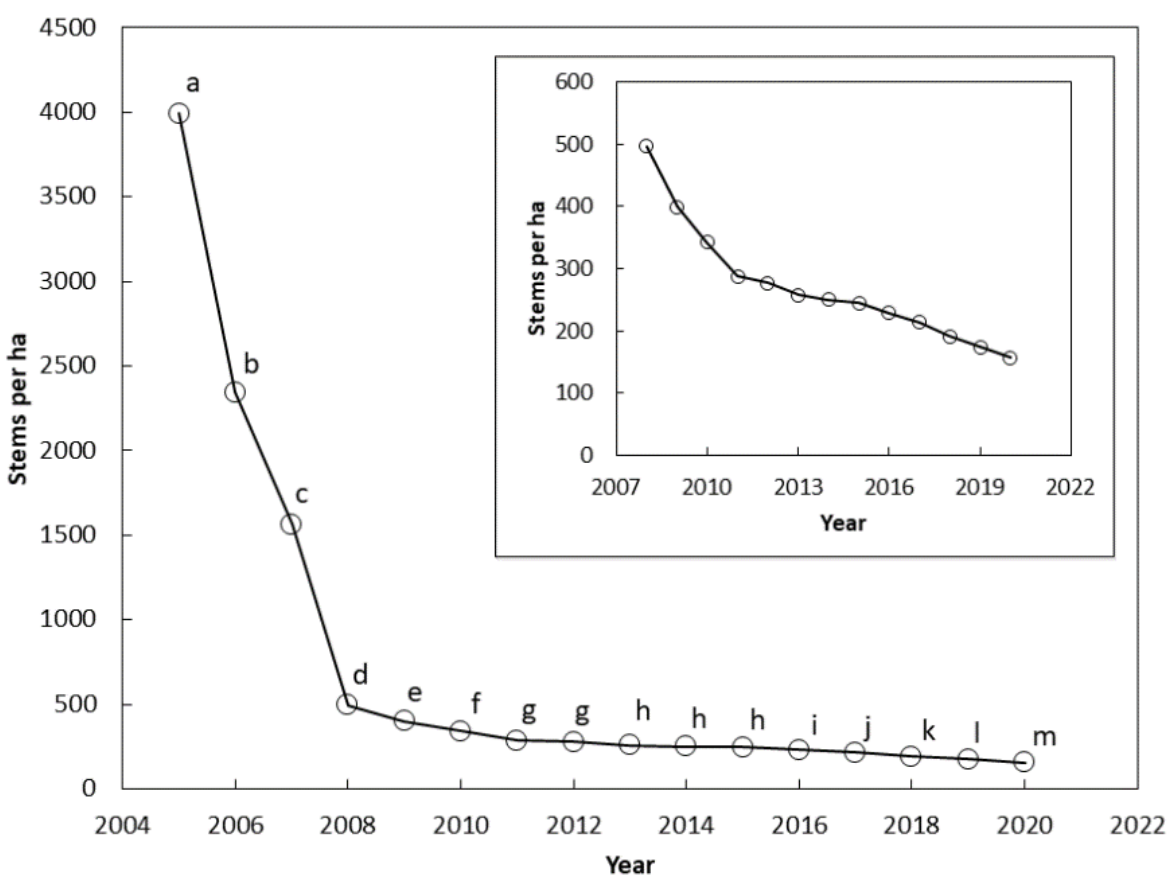
\includegraphics[width=\linewidth]{marler-stem-count}
	
	\caption{[From \cite{marlerLongitudeForestFragmentation2020}] The number
		of \textit{Cycas micronesica} stems per ha (all size categories) among 12 Guam habitats
		from 2005 until 2020. The inset shows results from 2008 until 2020 with smaller vertical axis range. Ordinates of markers with the same letter are not significantly different.}
	
	\label{fig:marler-stem-count}
\end{figure}


The Guam CAS outbreak, which was severe and spread rapidly throughout the island (Table \ref{tab:timeline}, Figure \ref{fig:marler-stem-count}), was well documented by Marler and others. Within 12 years, \textit{C. micronesica} went from being the most abundant tree in Guam's forests to being listed under the U.S. Endangered Species Act. It should be noted that since arrival of CAS, several other recently arrived invasive insect species and even some native species have begun attacking and damaging Guam's cycads (
\cite{marlerPestsCycasMicronesica2006}, \cite{mooreCoalitionInvasiveSpecies2013}, \parencite{delosoBioticThreatsCycas2020a}). 
However, CAS is considered to be the prime driver of population decline because it is the only herbivore causing damage severe enough to result in mortality.

Rapid decline of the Guam \textit{C. micronesica} population was documented by 
\cite{marlerLongitudeForestFragmentation2020} (Figure \ref{fig:marler-stem-count}). Data are annual cycad stem counts in 120 permanent plots established after infestation of Guam's wild cycads, but prior to any mortality. It can be seen in the figure that cycad stem count declined to only 12.5\% of the original within the first 3 years of the survey (2005-2008) and continued to decline to only 4\% of the original count in succeeding years (2009-2020). In addition to high plant mortality surviving cycads stopped reproducing in the Guam plots: the last seedling (0-10 cm tall) was seen in 2006 and the last juvenile (10-100 cm tall) was seen in 2014. Between 2014 and 2020 the annual mortality rate for mature plants was relatively stable at about 14 per ha.

\todo{Mention forest survey results here?}

\subsection{Impacts of CAS on \textit{C. micronesica} individuals}

Immediate impacts of CAS on health of \textit{C. micronesica} individuals is very obvious. On Guam, unprotected plants typically die within 18 months (REF) after being infested. Several overlapping generations of CAS totally encrust all leaves within a few months of infestation. Plant mortality is caused by a combination of nutrient removal by CAS sap feeding plus blockage of photosynthesis. Scales covers of dead insects are tightly affixed to the plant and these do not easily wash off. So photosynthesis may be blocked even after scale insects are killed. \cite{muniappanCycadAulacaspisScale2012} suggest that toxic effects of CAS saliva may also be involved in cycad mortality. 

%Impacts to plants infested with CAS linger after the scale insects have been killed by insecticides or biocontrol agents. Scale covers block photosysnthesis \parencite{tangReportRecommendationsCycad2005a}.

Secondary impacts of CAS on health of C. micronesica individuals are not obvious.

\subsubsection{Mature plants which have survived CAS infestation have reduced reproductive capacity}

Perhaps the most important secondary impact is much lower reproductive capability in plants recovering from CAS-infestation.  

\cite{marlerSourceSinkRelations2019} reported that seeds from CAS-infested plants are deficient in nonstructural carbohydrates  and germination rates are much lower: 43\% of seeds from healthy plants germinated versus 7\% of seeds from infested plants.

In addition, \cite{marlerAulacaspisYasumatsuiInvasion2021} reported that mature male plants which survived the initial CAS invasion have significantly smaller cones than prior to infestation. Average cone volume was 24\% of pre-infestation levels in 2007 and this increased to 57\% in 2021.

\subsubsection{Mature plants which have survived CAS infestation are more susceptible to typhoon damage}  

\textit{C. micronesica} and other endemic plants on Guam have evolved tolerence for typhoon strength winds (greater than 118 km/h) because tropical cyclones frequently visit this island.
\parencite{marlerIncreasedThreatIsland2013} reported on results of nondestructive winching stress tests performed on \textit{C. micronesica} stems to simulate effects of typhoon strength winds. Stems of plants which had not been infested by CAS were significantly stiffer than those which had been infested by CAS for either two or five years. Marler hypothesized from this finding that CAS-infested plants were much more susceptible to stem failure during typhoons.

Evidence supporting this hypothesis came two years after the original article was published, from a damage survey after Typhoon Dolphin passed over Guam on May 15, 2015.
\cite{marler2016topographic} compare the level of damage from Typhoon Dolphin with that of a previous cyclone, Supertyphoon Paka:
\begin{displayquote}
Supertyphoon Paka caused severe damage to
Guam’s forest resources in 1997 when the \textit{C. micronesica} population was
healthy and not threatened by any known invasive insect herbivores.
Less than 2\% of the healthy \textit{C. micronesica} population exhibited
windsnap damage during peak winds of 298 km/h. In contrast,
Typhoon Dolphin’s peak winds of only 170 km/h. caused windsnap
of 6\% (mean of our eight sampling sites) of Guam’s unhealthy \textit{C.
micronesica} population after only 10 years of \textit{A. yasumatsui} infestations.
\end{displayquote}
\textit{Windsnap} is synonymous with \textit{stem failure}. It is interesting to note that, because energy is a function of the square of wind speed, maximum winds generated by Paka were about 3 times more powerful than those of Dolphin.

\subsection{CAS-induced cascading impacts on Guam's forest ecosystems}

An \textit{ecological cascade effect} is a series of secondary extinctions that are triggered by the primary extinction of a key species in an ecosystem. \textit{C. micronesica} is considered to be a key species in Guam forest ecosystems because it was the most abundant tree prior to arrival of CAS. Loss of this plant is likely to threaten survival other organisms.

\subsubsection{Herbivores which depend on \textit{C. micronesica} for food} 

\paragraph{Marianus fruit bat, \textit{Pteropus mariannus}}

\cite{haynesExoticInvasivePest2005} reported:
\begin{displayquote}
The fleshy, aromatic covering of fadang seeds is a preferred food item for the endangered Mariana
fruit bat, \textit{Pteropus marianus marianus}. Fadang is so resistant to most types of disturbance that its
seeds are sometimes the only bat food item available in the forest following the destructive winds of a
passing cyclone. Fewer than 100 Mariana fruit bats remain on Guam and it is unknown what effect the
loss of fadang will have on these endangered bats.
\end{displayquote}

In 2020, the US Fish and Wildlife Service estimated that only 45 fruit bats remain on Guam in a single roost site on Andersen Air Force Base.

\paragraph{\textit{Dihammus marianarum} and \textit{Anatrachyntis} sp.}

\cite{marlerCanopyKnowledgeGaps2013} reported:
\begin{displayquote}
At least two arthropods	depend on the \textit{C. micronesica} population;
the endemic stem borer \textit{Dihammus marianarum} exploits cycad stem tissue for larval food, and the cone borer \textit{Anatrachyntis} sp requires microstrobili (male cones) for larval food.
\end{displayquote}

\textit{Dihammus marianarum} (=\textit{Acalolepta marianarum}) is an endemic longhorn beetle (Cerambicidae), which became a secondary pest of \textit{C. micronesica} after plants were infested with CAS. This beetle has many larval host plants \parencite{marlerPestsCycasMicronesica2006} so \textit{C. micronesica} is probably not critical for its survival.

On the other hand the cosmopterigid moth, \textit{Anatrachyntis} sp, has been identified as a probable pollinator of \textit{C. micronesica} and it has been suggested that this insect may be an obligate symbiont, meaning that it cannot survive without the cycad. 

An abundance of larvae are found in every
male cone following pollen shedding. Pupation takes place in a silken cocoon on the surface of the cone \parencite{marlerPestsCycasMicronesica2006}.
\cite{terryConeInsectsPutative2009} used sticky traps to sample insects and pollen in the vicinity of \textit{Cycas micronsica} cones. They reported:

\begin{displayquote}
	On female cone sticky traps, ~30\% of the
	pollen grains were associated with Anatrachyntis moths or moth scales
	and less than 5\% with other insects; however, over 60\% of the pollen
	was not associated with any insect, suggesting some pollen is wind
	dispersed.
\end{displayquote}

Based on these observations, they hypothesized that \textit{C. micronesica} is pollinated both by wind and insects, with \textit{Anatrachyntis} sp being an important insect pollinator.

No lepidopteran had previously been identified as a cycad pollinator. However, nine years later \cite{huaFirstRecordAnatrachyntis2018} reported that a moth in the same genus, \textit{Anatrychintis badi}, was discovered feeding in male cones of a native Florida cycad, \textit{Zamia integrifolia}, and suggested that this species may also be an insect pollinator.

Details of the hypothesized symbosis between the unidentified \textit{Anatrachyntis} species and \textit{C. micronesica} on Guam are not fully understood. The relationship between partners in this symbiosis differs markedly from than between flowering plants and their insect pollinators:
\begin{enumerate}
	\item The reward for pollination service is provided to the caterpillar stage by the male plants which provide food in the form of sacrificial tissues within the male cone. The male cone may also provide a site free from competitors and natural enemies. The presumption here is that the caterpillars are protected by cycad toxins to which they have evolved tolerance.
	\item There is no known reward provided to adults moths carrying pollen to female cones for pollination to take place. It is not known how \textit{Anatrahynitis} moths are attracted to female cones of \textit{C. micronesica}. 
\end{enumerate}

The biology of \textit{Atrachyntis} on Guam is largely unknown apart from its association with \textit{C. micronesica}. It is possible that this species is highly specialized and that its survival is totally dependent on availability of male cones. Alternatively, it is possible that this moth is not an obligate symbiont, but has broad host range.  

\subsubsection{Ecosystem services provided by \textit{C. micronesica}}

\paragraph{Nitrogen fixation and impacts on forest soils}

\textit{C. micronesica} is the only dominant native tree on Guam which nitrogen-fixing sympionts. Therefor, the native biota of Guam's habitats has developed with this living resource provisioning the ecosystem with nitrogen. \parencite{marlerArthropodInvasionDisrupts2011}. In the case of cycads, the nitrogen fixing symbionts are cyanobacteria groowing in specialized structures called coralloid roots.  

\subsubsection{Prognosis for Guam's Forests} 

Currently, mature \textit{C. micronesica} in Guam's forests are dying and these are not being replaced by seeds or juvenile plants. It is obvious that without a change, this endemic plant, the most abundant tree in Guam's forests only two decades ago, is headed towards local extinction.

Pending extirpation of Guam's native cycads is not the first or last ecological disaster caused by invasive species in Guam's forests \parencite{moore_failed_2018}. The brown tree snake, \textit{Boiga irregularis}, first detected in 1953 caused extinction or extirpation of all Guam's forest birds, also removing the ecosystem services they provided such as seed disperal, insectivory, and pollination. The coconut rhinoceros beetle, \textit{Oryctes rhinoceros}, first detected in 2007 is killing large numbers of coconut palms, \textit{Cocus nucifera}, and the introduced palma brava, \textit{Heterospathe elata}. These palm species were identified as Guam's second and third most abundant trees in the 2002 forestry survey. \parencite{donnegon_guams_2004}.

Restoration of Guam's forests to their pristine state is no longer possible. However, there is an urgent need to control CAS and other key invasive species so that some recovery can take place, without further loss of biodiversity. 

\section{Natural enemies of CAS - Cave}

\section{Classical biological control}

\subsection{Florida - Cave}

\subsection{Hawaii - Wright}

\subsection{Guam - Moore}

\subsubsection{\textit{Rhyzobius lophanthae}}

About 100 adults of \textit{Rhyzobius lophanthae} were field collected on Maui and imported to Guam during November 2004. This coccinelid was originally 
introduced to California from Australia in 1892 and to Hawaii from California in 1894. It was observed feeding voraciously on CAS shortly after arrival of this new pest in Hawaii. 

\textit{R. lophanthae} was previously introduced to Guam on two separate occasions under various synonyms: \textit{R. satelles} Blackburn, \textit{Lindorus lophanthae} (Blaisdell), and \textit{R. pulchellus} Montrouzier (\cite{nafus_biological_1989}).
In 1925 and 1926 \textit{Rhyzobius satelles} was imported to Guam from California to control the coconut scale, \textit{Aspidiotus destructor} Signoret. However, attempts at field establishment failed.  

\cite{nafus_biological_1989} also reported:
\begin{displayquote}
 In 1971, \textit{Rhyzobius satelles} Blackburn (as \textit{R. pulchellus} Montrouzier) was introduced to Guam from New Caledonia to aid in the control of coconut scales and citrus scales. A single specimen of \textit{R. satelles} was recovered in 1978, indicating establishment. The beetle, however, is very uncommon; an intensive survey of coconut insects in 1984 yielded no specimens.
\end{displayquote}

The beetles from Maui were reared on scale-infested \textit{C. micronesica} cuttings placed in a large screened camping tent set up in a laboratory. Adult offspring were collected for field release by aspirating them from the walls of the tent into plastic vials. Field releases were initiated on February 16 2005 at the Guam National Wildlife Refuge at Ritidian Point. The beetles established readily. By July 7 2005 high densities on adults were observed on cycads anywhere within a 1 km radius of the release site.  Establishment and dispersion of the beetles were monitored using yellow sticky traps deployed between June 2005 and May 2006. Unexpectedly, we were also able to monitor CAS crawlers and adult males using these traps (Fig. \ref{fig:sticky-traps})  (\cite{moore_biological_2017-2}). Following establishment of \textit{R. lophanthae} at Ritidian Point, laboratory-reared and field-collected beetles were released at about 30 other sites throughout Guam. 

\begin{figure}[H]
	\centering
	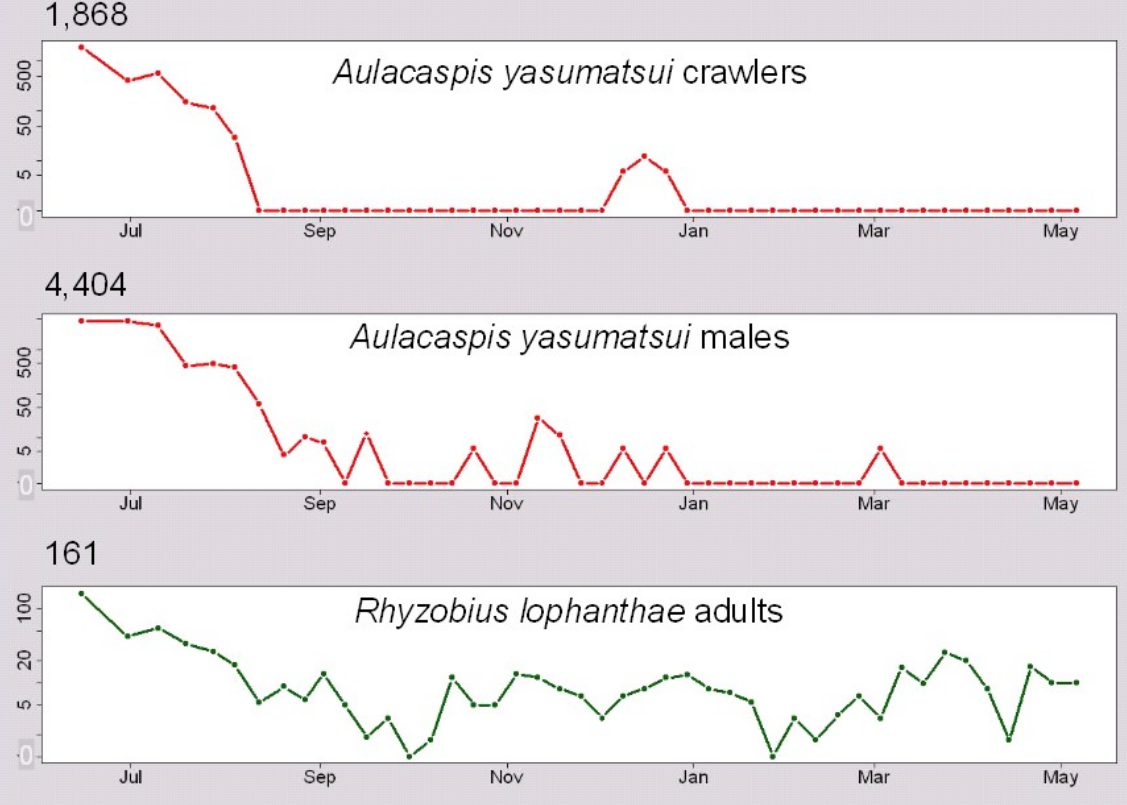
\includegraphics[width=\linewidth]{sticky-traps1}
	
	\caption{Insects trapped on yellow sticky cards at Ritidian Point, Guam following field release of Rhyzobius lophanthae in February, 2005. X axis runs from July 2005 through May 2006; Y-axis, in log scale, is number of insects trapped per square meter per day. [Figure from \cite{moore_biological_2013-2}]}
	
	\label{fig:sticky-traps}
\end{figure}

By about 2010, \textit{R. lophanthae} larvae or adults could be found on almost every CAS-infested cycad on Guam, preventing CAS from killing mature cycads. By 2010, about 90\% of wild cycads had been killed on Guam (REF). Unfortunately, the \textit{C. micronesica} population is not recovering because almost all seeds and seedlings are being killed by CAS and other causes (REF). \cite{marlerVerticalStratificationPredation2013} showed that \textit{R. lophanthae} predation of CAS is significantly reduced close to the ground and suggest that this may partially account for failure of the beetle to protect CAS seedlings. They also suggested:
\begin{displayquote}
The causes of reduced scale predation by
\textit{R. lophanthae} near the ground are unknown,
but a parasitoid biological control agent may
not exhibit these same limitations. Furthermore, because a parasitoid would be much
smaller than \textit{R. lophanthae}, it would likely be
better able to access scale infestations within
cracks and crevices on \textit{C. micronesica} and
\textit{C. revoluta} trees.
\end{displayquote}

\subsubsection{\textit{Coccobius fulvus}}  

\subsubsection{\textit{Aphytis lignanensis}}

\subsubsection{\textit{Arrhenophagus}}  

Ask Mark, Janis about Bernarr's report on fortuitous introduction of CAS parasitoids.

Ask Reddy about his report.

Ask Arnold Harra.


\subsection{Elsewhere - Cave}

\section{Prospects for future action - Cave, Wright, and Moore}

\newpage
\printbibliography[heading=bibintoc]

\begin{appendices}
	
	Notes from key references.

\section{Haynes and Marler 2005}

\subsection{fadang plants provide crucial food for other organisms}
\begin{displaycquote}{haynesExoticInvasivePest2005}
A second reason for funding this project is that fadang plants provide crucial food for other organisms.
The fleshy, aromatic covering of fadang seeds is a preferred food item for the endangered Mariana
fruit bat, Pteropus marianus marianus. Fadang is so resistant to most types of disturbance that its
seeds are sometimes the only bat food item available in the forest following the destructive winds of a
passing cyclone. Fewer than 100 Mariana fruit bats remain on Guam and it is unknown what effect the
loss of fadang will have on these endangered bats. (For more information on Guam’s fruit bats, refer
to the following website: http://www.fws.gov/pacific/pacificislands/wesa/marianabatindex.html.)
We have only just begun our herbivory surveys of Cycas micronesica. In our preliminary work, we
have identified the indigenous stem borer, Dihammus marianarum (Coleoptera: Cerambycidae), as a
common cycad consumer. When these surveys are completed, there may be other native arthropod
cycad consumers. Thus, the loss of this host species may also lead to the loss of several native species.
\end{displaycquote}

\subsection{symbiotic relationships}
\begin{displaycquote}{haynesExoticInvasivePest2005}
A third reason this project deserves emergency status is that cycad plants are part of a tripartite
symbiotic system of organisms. As with many species of plants, cycad roots are invaded by
mycorrhizal fungi. However, cycads also produce coralloid roots that are host to nitrogen-fixing
cyanobacteria. Work in ex-situ sites reveals that any available genotype of cyanobacteria can invade
coralloid roots. This is also probably true for mycorrhizae. Thus, determining the genetic variation of
cycad mycorrhizae and cyanobacteria in the native habitat is needed to shed light on conservation of
these important organisms. Loss of Cycas micronesica from Guam’s various populations could easily
result in the permanent loss of local genotypes of these other organisms that make up this complex,
interconnected system.
\end{displaycquote}

\subsection{pollinator(s)}
\begin{displaycquote}{haynesExoticInvasivePest2005}
A fourth reason for considering this a top priority for emergency funding is the nature of cycad
pollination dynamics. We now know that cycads are pollinated almost exclusively by obligate insect
pollinators (Norstog \& Nicholls, 1997; Whitelock, 2002). We are attempting to identify the insect(s)
which co-evolved with Guam’s cycad population as the pollinators. At the present time, so many of
the habitats are infested with CAS that it is difficult to find individual cycads suitable for pollination
studies. The probability of one or more endemic, obligate insect pollinators occurring on Guam is
highly likely. These beneficial insects will also be lost along with Guam’s cycad population should we
continue to stand by and let the CAS epidemic continue unchecked.
\end{displaycquote}

\subsection{fadang is an iconic plant}
\begin{displaycquote}{haynesExoticInvasivePest2005}
Our height increment data indicate that many of Guam’s coastal cycad plants are hundreds of years
old. These plants have survived the Spanish-American War and two world wars; they have survived
innumerable tropical cyclones; they have survived the invasion of intentionally introduced feral deer
and pig populations and the accidental introduction of various insect species. Some of these individual
plants “watched” Ferdinand Magellan and his fleet sail along Guam’s coast on 6 March 1521. And
they endured the Spanish-Chamorro Wars that decimated the indigenous human population. Truly, the
remaining plants comprise a long-lived botanical and cultural treasure, one that is in danger of
disappearing forever. We simply cannot elect to continue to watch this tragedy without attempting to
intervene. The impending cascade of detrimental effects is looming too large to justify apathy.
\end{displaycquote}

\section{2005 - Report and recommendations on cycad aulacaspis scale}

\subsection{list of known CAS biocontrol agents}
\begin{displaycquote}{tangReportRecommendationsCycad2005a}
BIOLOGICAL CONTROL

In practice, the introduction of predators or parasitoids is the most cost- and labor-effective method of
controlling scale insect infestations. It is also the standard approach for long-term control of introduced
exotic scale pests (Meyerdirk, 2002). The existence of effective natural biocontrol agents for CAS can be
assumed, since the scale is usually in low or moderate densities in wild populations of Cycas in Thailand,
where CAS is native, where it does not cover foliage like it does in cultivated plants (Tang et al., 1997).
At least three such predators or parasitoids have been identified and tested in the field as biocontrol agents
for CAS.
In 1996, Dr. Richard Baranowski of the University of Florida-Homestead (retired), working with Banpot
Naponpeth, director of the Natural Biological Control Research Center at Kawetsart University in
Bangkok, Thailand, identified two potential biocontrol organisms. This research was conducted in part on
the grounds of Nong Nooch Tropical Garden. Both insects were evaluated and then widely released in
Florida as biocontrol agents of CAS.
Coccobius fulvus (Compere \& Annecke) (Hymenoptera: Aphelinidae) is a parasitoid 3 wasp no larger than its
host, ca. 1 mm long (see Fig. 1). Observations of this organism in south Florida suggest that this wasp, by itself,
is not aggressive enough to control CAS on Cycas plants, such as C. revoluta, that are highly susceptible to
CAS (Caldwell, 2005), but it can be effective in large, heavily infested plants of other Cycas species and/or
plants with dense foliage in which pesticide application is inhibited (Wiese et al., in press). Coccobius fulvus
has also been released as a biocontrol agent of other diaspid scale insects in the U.S. (Meyerdirk, 2002).
Cybocephalus binotatus Grouvelle (Coleoptera: Nitidulidae) is a predatory beetle not much longer than CAS
(see Fig. 2). The adult punctures the scale cover and chews on the living scale underneath; it will also deposit
eggs under the scale cover, where its larvae then feed on CAS eggs. A study of the effects of this predator on a
similar species of Aulacaspis on mangos suggests that, because it requires a substantial scale population to
maintain effective numbers, it must be re-released periodically into infested areas to maintain effective control
(Lagadec, 2004). Thus, an active, ongoing release program may be necessary for effective control using this
biocontrol agent. Recently the beetle released in Florida has been re-identified as Cybocephalus nipponicus
(Endrody-Younga) (R. Cave, pers. comm.).
The ladybird beetle, Rhyzobius lophanthae (Blaisdell) (Coleoptera: Coccinellidae), a native of Australia
that is often called the “scale destroyer,” has been successfully used as a control agent for CAS on
cultivated Cycas plants in Hawaii by the University of Hawaii and the Hawaii Department of Agriculture
(Hara et al., undated). It has also been reared and released on Guam since February 2005 to combat the
CAS infestation in wild Cycas micronesica populations. This beetle seems to be taking hold and
spreading on Guam, but effective control of CAS has not yet been achieved to date (A. Brooke \& I. Terry,
pers. comm.). Although this beetle was established in Florida as a predator of other scale insects prior to
the outbreak of CAS, it has not been observed to have any significant impact on CAS infestations (R.
Cave, pers. comm.). To be effective, this predator must be reared and released in significant numbers in
infested areas and re-released as outbreaks reoccur.
Other potential biocontrol agents have been identified or suggested, but these require more surveys in the
wild, in addition to subsequent lab and field evaluations, before their effectiveness will be known. They
include insects, mites, and fungi.
Insects
The twice stabbed lady beetle, Chilocorus stigma (Say), a species native to the U.S., has been observed
feeding on CAS on cultivated Cycas in Florida (Cave \& Duetting, 2004; Tang \& Skarlinsky, unpubl.).
Again, observations suggest that, to be effective, such coccinellid beetles require repeated mass release in
infected areas. This species is a generalist that attacks a variety of diaspids.
The following parasitoids of the wasp families Aphelinidae and Encyrtidae have been identified in
southern China and Vietnam and may have potential as biocontrol agents of CAS (Cave, unpubl.;
Meyerdirk, 2002):
•
•
3
Aprostocetus sp. (possibly A. purpuratus
Girault)
Arrhenophagus sp. (possibly A. chionaspidis
Aurivillius)
•
•
•
•
Aphytis lepidosaphes Compere
Encarsia sp.
Pteroptrix chinensis (Howard)
Thomsonisca sankarani Subba Rao

Mites
The mite, Hemiarcoptes sp. (prob. H. coccophagus), has been found to control a related species of
Aulacaspis in a lab setting (Meyerdirk, 2002).
Fungi
An unidentified fungus is known to grow on masses of the scale, Aulacaspis tegalensis (Zehntner)
(Meyerdirk, 2002). Another unidentified fungus has been observed growing on CAS in Florida (Caldwell,
2005).
\end{displaycquote}

\subsection{CAS is fatal}

\begin{displaycquote}{tangReportRecommendationsCycad2005a}
CAS will kill an infected Cycas host plant within a year if no control measures
are taken.
\end{displaycquote}

\subsection{Primary Recommendations to the CSG}
\begin{displaycquote}{tangReportRecommendationsCycad2005a}
To reiterate, the activities of major urgency that the CSG should pursue are the following:

1. A major priority must be to promote research on identifying new biocontrol agents for CAS and
determining how to improve the effectiveness and accelerate the establishment of biocontrol organisms
in newly infested areas.

2. Work together with the IUCN/SSC Invasive Species Specialist Group and the Global Invasive Species
Programme to alert plant protection organizations of countries throughout the tropics and subtropics—
especially those that possess wild species of Cycas—about the threat of CAS. Provide them with
information and techniques for effective exclusion of CAS. This will require tapping into the IUCN
and/or other high profile media outlets.

3. Assist with locating funding for current control efforts in Guam and Taiwan. Aid in collating and
documenting such efforts, so as to identify the most effective techniques and avoid repeated
duplication of ineffective control measures.
\end{displaycquote}

\end{appendices}


\end{document}
